
\section{Introduction}
Millions of people worldwide suffer from asthma, a chronic respiratory disease. Breathing becomes difficult as a result of episodes of airway inflammation and constriction. For asthma to be effectively managed and treated, severity classification must be done accurately. Conventional diagnostic techniques, such as subjective evaluations and physical exams, might not be as accurate as they need to be for the best possible treatment planning.

The goal of this study is to utilize machine learning (ML) to categorize asthma severity levels using patient data. Our goal is to create a system that improves diagnostic precision, permits prompt treatments, and aids medical professionals in making well-informed decisions by employing a data-driven approach. The system predicts the severity of asthma and provides accurate treatment recommendations by analyzing a number of variables, such as patient demographics, medical history, spirometry findings, and symptom frequency.

To guarantee strong classification performance, the suggested system incorporates a variety of machine learning methods, including Random Forest, Support Vector Machines (SVM), and Logistic Regression. The method saves diagnostic time and human error by automating the prediction process, which eventually improves asthma management and patient outcomes.

\subsection{Motivation}
The increasing incidence of asthma and the difficulties medical professionals encounter in properly diagnosing and treating the condition are the driving forces behind this research. Determining the best course of treatment requires an accurate and rapid classification of asthma severity, but traditional diagnostic techniques frequently rely on manual patient data interpretation and subjective clinical assessments.

As electronic health records (EHRs) become more widely available and medical data volumes increase, machine learning presents a chance to transform asthma diagnosis through the use of unbiased, data-driven insights. Healthcare professionals can give patients with better individualized care by receiving quick, accurate, and trustworthy forecasts by automating the asthma classification process.

Furthermore, a major driving force behind this effort is the possibility that machine learning may continue to advance over time as a result of exposure to fresh data and feedback. Asthma sufferers' quality of life may increase as a result of more efficient asthma management techniques brought about by the system's capacity to adjust and improve its accuracy.

\subsection{Methodology}
A methodical procedure was used to create the Asthma Disease Classification System. To guarantee consistency and quality, patient data was gathered and preprocessed, including demographic information, medical history, and clinical test results. To categorize the severity of asthma, machine learning algorithms including Support Vector Machines, Random Forest, and Logistic Regression were trained using historical patient data. Reliability was ensured by evaluating the models using accuracy and F1-score. In the end, the system was implemented as a safe and intuitive web application that protected patient data while giving medical experts real-time forecasts.
\subsection{Outcomes}
Asthma severity levels were accurately defined using the Asthma Disease Classification System, allowing for prompt and accurate diagnosis. By lowering manual errors and improving healthcare workers' decision-making, the use of machine learning models increased diagnostic precision. Clinical operations were eased by the intuitive web application, which offered thorough insights and real-time forecasts. Sensitive patient data was also protected by strong security measures, which made the system reliable and efficient for everyday use.

\section{Codes}
\subsection{Import Data}
\begin{verbatim}
import pandas as pd
import numpy as np
import matplotlib.pyplot as plt
df=pd.read_csv(r"C:\Users\varun\Downloads\asthma_disease_data.csv")
df
\end{verbatim}
\subsection{Data Columns and Shape}
\begin{verbatim}
df.columns
Output:Index(['PatientID', 'Age', 'Gender', 'Ethnicity', 
'EducationLevel', 'BMI', 'Smoking', 'PhysicalActivity', 
'DietQuality', 'SleepQuality','PollutionExposure', 
'PollenExposure', 'DustExposure', 'PetAllergy',
'FamilyHistoryAsthma', 'HistoryOfAllergies',
 'Eczema', 'HayFever','GastroesophagealReflux',
 'LungFunctionFEV1', 'LungFunctionFVC', 'Wheezing', 
'ShortnessOfBreath', 'ChestTightness', 'Coughing',
'NighttimeSymptoms', 'ExerciseInduced',
 'Diagnosis', 'DoctorInCharge'],dtype='object')
df.shape
(2392, 29)
\end{verbatim}
\subsection{Visualization}
\subsubsection{Gender Distribution (Bar Chart)}
\begin{verbatim}
df['Gender'].unique()
gen=df['Gender'].value_counts()
x=gen.index
y=gen.values
plt.figure(figsize=(6,4))
plt.title('Gender Distribution')
plt.bar(x,y,color=['black','pink','red'])
plt.xlabel('Gender')
plt.ylabel('Counts')
plt.show()
\end{verbatim}

\textbf{Ouput:}
\begin{figure}[h]
\centering
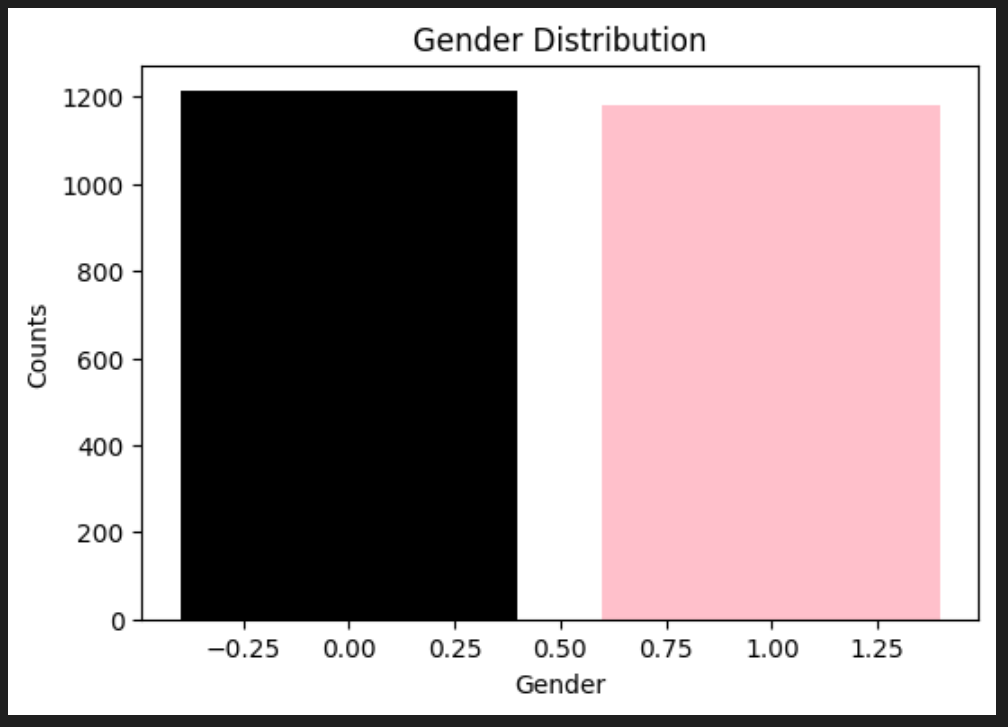
\includegraphics[width=0.7\linewidth]{Images/1.png}
\caption{Bar chart}
\label{fig:enter-label}
\end{figure}
The gender distribution in the dataset is displayed in the first figure using a bar chart. The number of individuals is displayed on the y-axis, while gender is displayed on the x-axis. The black bar most likely represents the male gender category, whereas the pink bar most likely represents the female gender category. The figure demonstrates that the counts are almost similar for both genders, with a little higher count in the pink category. Since the gender axis labels (such as 0 and 1) are not obvious, it would be helpful to specifically designate the categories (such as "Male" and "Female") for easier comprehension.

\subsubsection{Education Level Distribution (Pie Chart)}
\begin{verbatim}
df['EducationLevel'].unique()
edu=df['EducationLevel'].value_counts()
x=edu.index
y=edu.values
plt.figure(figsize=(6,4))
plt.title('Education Level Distribution')
plt.pie(y,labels=x)
plt.legend(x,loc="upper right")
plt.show()
\end{verbatim}

\textbf{Ouput:}
\begin{figure}[h]
\centering
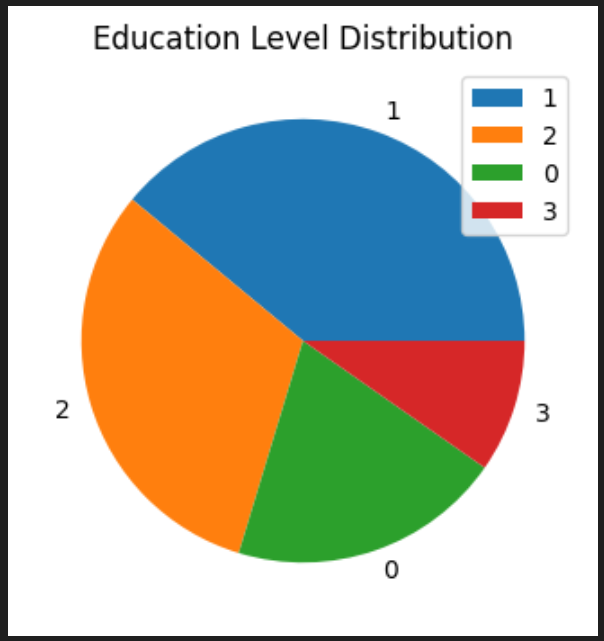
\includegraphics[width=0.7\linewidth]{Images/g2.png}
\caption{Pie Chart}
\label{fig:enter-label}
\end{figure}
The subsequent graphic uses a pie chart to display the distribution of education levels within the dataset. The legend states that each component stands for a different educational level: Red is represented by three, orange by two, and green by zero. Education levels "0" (green) and "3" (red) have lesser proportions than levels "1" (blue) and "2" (orange), according to the chart. This suggests that most people in the dataset have intermediate education levels (represented by 1 and 2), but basic (0) and higher education (3) levels are less prevalent. The distribution's obvious legend and markings make it simple to understand.

\subsubsection{ Age Distribution (Histogram)}
\begin{verbatim}
df['Age'].min()
df['Age'].max()
x=df['Age']
plt.figure(figsize=(8,6))
plt.title('Age Distribution')
plt.hist(x,bins=[10,20,30,40,50,60,70,80],color='yellow')
plt.xlabel('Age')
plt.ylabel('Counts')
plt.show()
\end{verbatim}
\textbf{Ouput:}
\begin{figure}[h]
\centering
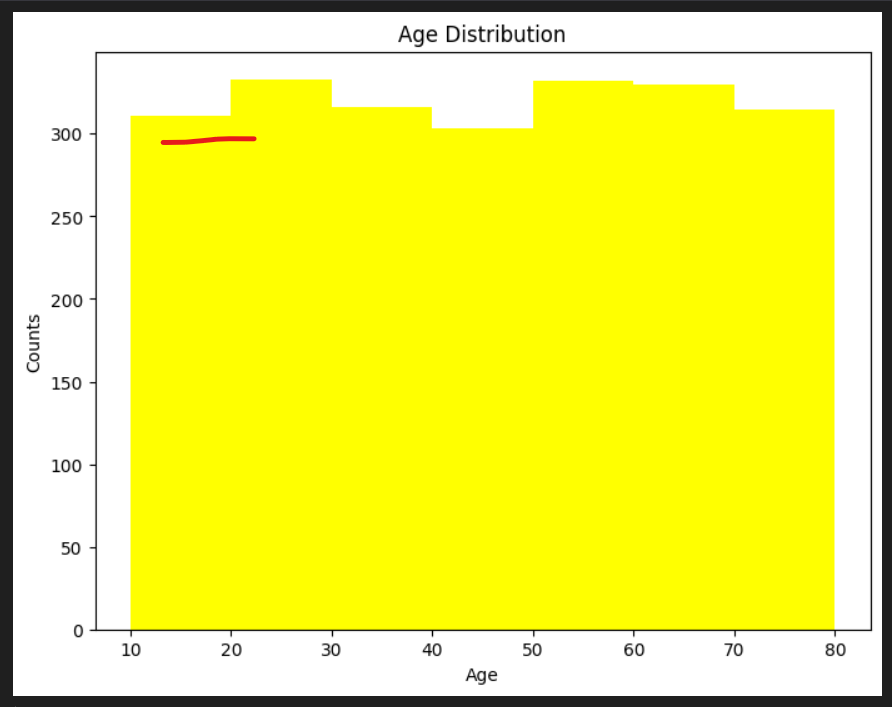
\includegraphics[width=0.7\linewidth]{Images/g1.png}
\caption{Histogram}
\label{fig:enter-label}
\end{figure}
 displays the age distribution of individuals using a histogram. The x-axis displays the age range, and the y-axis displays the number of individuals in each age bin. The data appears to be evenly distributed across the age range (10 to 80 years), as most bins contain almost equal numbers (approximately 300 people). This suggests that different age groups are fairly represented in the sample. Even while the bright yellow of the bars makes them visible, choosing a less bright tint might improve their aesthetic appeal. Adding more thorough age bin labels on the x-axis would further increase readability.

\subsection{Splitting Data}
\begin{verbatim}
from sklearn.model_selection import train_test_split
x_train,x_test,y_train,
y_test=train_test_split(x,y,test_size=0.2,random_state=42)
x_test.shape
x_train.shape
y_train.shape
y_test.shape
\end{verbatim}

\subsection{LogisticRegression Algorithm}
\begin{verbatim}
from sklearn.linear_model import LogisticRegression
from sklearn.metrics import accuracy_score,confusion_matrix
from sklearn.preprocessing import StandardScaler
import seaborn as sns
lr=LogisticRegression()
lr.fit(x_train,y_train)
predict_lr=lr.predict(x_test)
predict_lr
accuracy=accuracy_score(y_test,predict_lr)
accuracy
cm=confusion_matrix(y_test,predict_lr)
cm
y_test
sc= StandardScaler()
x_train=sc.fit_transform(x_train)
x_test=sc.transform(x_test)
x_train
x_test
train_score=lr.score(x_train,y_train)
train_score
train_score=lr.score(x_test,y_test)
train_score
plt.figure(figsize=(8,4))
plt.title('confusion matricx')
sns.heatmap(cm,annot=True,fmt='d')
plt.xlabel('True value')
plt.ylabel('predicted value')
plt.show()
\end{verbatim}
\textbf{Ouput:}
\begin{figure}[h]
\centering
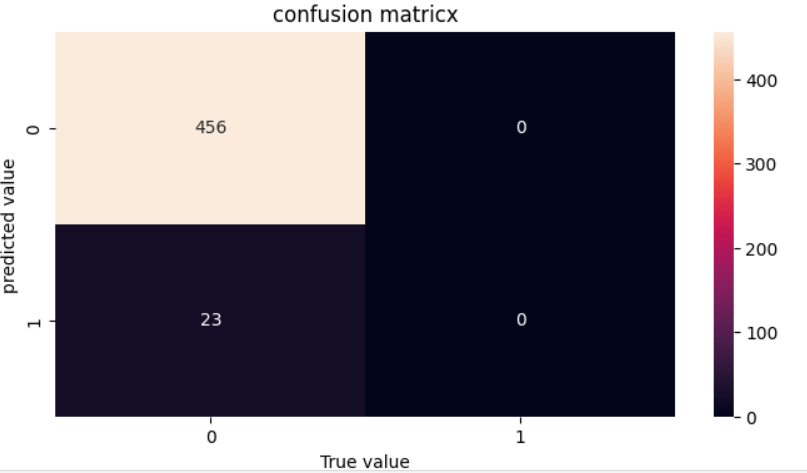
\includegraphics[width=0.7\linewidth]{Images/r1.png}
\caption{HeatMap(LogisticRegression Algorithm)}
\label{fig:enter-label}
\end{figure}
By correctly identifying 456 non-asthma cases but failing to predict any asthma cases, with 23 false negatives and no true positives, the confusion matrix assesses the model's performance in predicting asthma. This suggests that the model is biased towards predicting "No Asthma" and has trouble identifying actual asthma cases, most likely as a result of class imbalance or insufficient sensitivity.

\subsection{DecisionTreeClassifier Algorithm}
\begin{verbatim}
from sklearn.tree import DecisionTreeClassifier
from sklearn.metrics import accuracy_score,confusion_matrix
import seaborn as sns
dcl=DecisionTreeClassifier()
dcl.fit(x_train,y_train)
predict_dcl=dcl.predict(x_test)
predict_dcl
accuracy=accuracy_score(y_test,predict_dcl)
accuracy
cm=confusion_matrix(y_test,predict_dcl)
cm
y_test
train_score=dcl.score(x_train,y_train)
train_score
train_score=dcl.score(x_test,y_test)
train_score
plt.figure(figsize=(8,4))
plt.title('confusion matricx')
sns.heatmap(cm,annot=True,fmt='d')
plt.xlabel('True value')
plt.ylabel('predicted value')
plt.show()
\end{verbatim}
\textbf{Ouput:}
\begin{figure}[h]
\centering
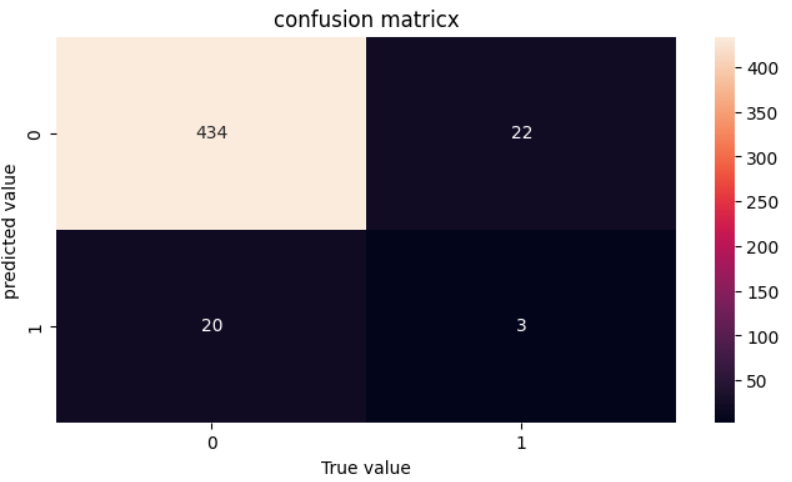
\includegraphics[width=0.7\linewidth]{Images/r3.png}
\caption{HeatMap(DecisionTreeClassifier Algorithm)}
\label{fig:enter-label}
\end{figure}
The confusion matrix demonstrates that while the model successfully predicts 434 non-asthma cases, it has trouble detecting asthma, correctly categorizing 20 asthma cases as non-asthma and only detecting three true positives. Furthermore, it misclassifies 22 occurrences of non-asthma as asthma, suggesting an imbalance between sensitivity and precision.\textbf{Above all algorithm Decision Tree Classifier give more accurate result}.

\subsection{RandomForestClassifier Algorithm}
\begin{verbatim}
from sklearn.ensemble import RandomForestClassifier
import seaborn as sns
rn=RandomForestClassifier()
rn.fit(x_train,y_train)
predict_rn=rn.predict(x_test)
predict_rn
y_test
accuracy=accuracy_score(y_test,predict_rn)
accuracy
cm=confusion_matrix(y_test,predict_rn)
cm
train_score=rn.score(x_train,y_train)
train_score
train_score=rn.score(x_test,y_test)
train_score
plt.figure(figsize=(8,4))
plt.title('confusion matricx')
sns.heatmap(cm,annot=True,fmt='d')
plt.xlabel('True value')
plt.ylabel('predicted value')
plt.show()
\end{verbatim}
\textbf{Ouput:}
\begin{figure}[h]
\centering
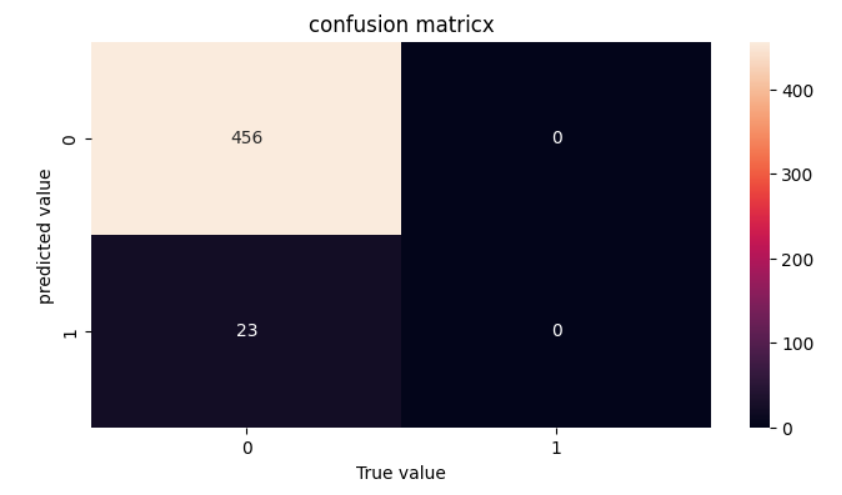
\includegraphics[width=0.7\linewidth]{Images/r2.png}
\caption{HeatMap(RandomForestClassifier Algorithm)}
\label{fig:enter-label}
\end{figure}
The confusion matrix evaluates how well the model predicts asthma. It shows that although the model correctly identifies 456 non-asthma cases, it cannot predict any asthma patients, as evidenced by the 23 false negatives and the lack of true positives. This implies that the model is biased toward predicting "No Asthma" and struggles to identify actual asthma patients, most likely due to class imbalance or low sensitivity.

\subsection{SVC Algorithm}
\begin{verbatim}
from sklearn.svm import SVC
import seaborn as sns
sc=SVC()
sc.fit(x_train,y_train)
predict_sc=sc.predict(x_test)
predict_sc
y_test
accuracy=accuracy_score(y_test,predict_sc)
accuracy
cm=confusion_matrix(y_test,predict_sc)
cm
df.isna().sum()
df.info()
plt.figure(figsize=(8,4))
plt.title('confusion matricx')
sns.heatmap(cm,annot=True,fmt='d')
plt.xlabel('True value')
plt.ylabel('predicted value')
plt.show()
\end{verbatim}
\begin{figure}[h]
\centering
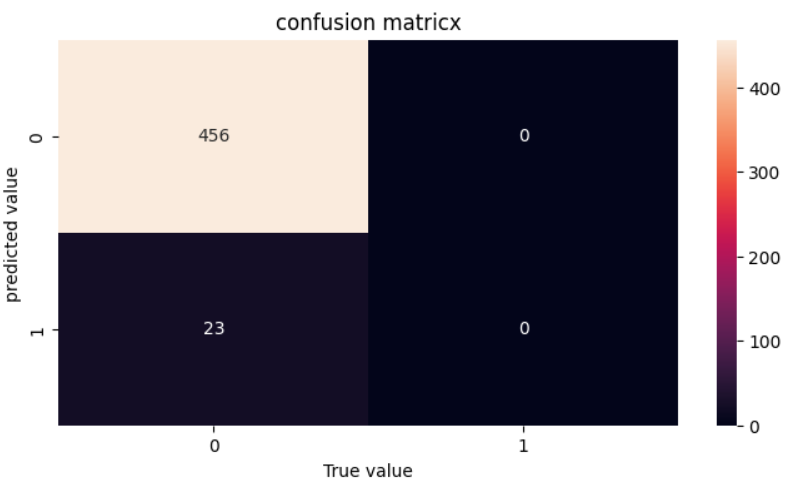
\includegraphics[width=0.7\linewidth]{Images/r4.png}
\caption{HeatMap(SVC Algorithm)}
\label{fig:enter-label}
\textbf{Ouput:}
\end{figure}
The model's asthma prediction accuracy is evaluated by the confusion matrix. It shows that although the model correctly identifies 456 non-asthma cases, it cannot predict any asthma patients, resulting in 23 false negatives and no true positives.

\subsection{Main File}
\begin{verbatim}
from flask import Flask, render_template, request
import pandas as pd
import pickle

# Load the pre-trained model
with open('a_model.pkl', 'rb') as model_file:
    model = pickle.load(model_file)

# Load the pre-trained scaler (used during training)
with open('nr_model.pkl', 'rb') as scaler_file:
    scaler = pickle.load(scaler_file)

# Initialize Flask app
app = Flask(__name__)

# Define the input features for the model
input_columns = [
    'Age', 'Gender', 'BMI', 'Smoking', 
    'PhysicalActivity', 'DietQuality', 'SleepQuality',
    'FamilyHistoryAsthma', 'LungFunctionFEV1',
     'LungFunctionFVC', 'Wheezing','ShortnessOfBreath'
]
# Route to display the form and handle user input
@app.route("/", methods=["GET", "POST"])
def index():    
    if request.method == "POST":
        # Extract the user input data
        user_input = {
            'Age': int(request.form['Age']),
            'Gender': request.form['Gender'],
            'BMI': float(request.form['BMI']),
            'Smoking': request.form['Smoking'],
            'PhysicalActivity': request.form['PhysicalActivity'],
            'DietQuality': request.form['DietQuality'],
            'SleepQuality': request.form['SleepQuality'],
            'FamilyHistoryAsthma':request.form['FamilyHistoryAsthma'],
            'LungFunctionFEV1':float(request.form['LungFunctionFEV1']),
            'LungFunctionFVC':float(request.form['LungFunctionFVC']),
            'Wheezing':request.form['Wheezing'],
            'ShortnessOfBreath':request.form['ShortnessOfBreath']
        }
        # Convert user input into a DataFrame
        input_df = pd.DataFrame([user_input])

        # Scale the input data using the pre-trained scaler
        input_scaled = scaler.transform(input_df[input_columns])

        # Make prediction
        prediction = model.predict(input_scaled)

        # Display prediction result
        diagnosis = 'Asthma' if prediction[0] == 1 else 'No Asthma'

        return render_template('result.html', diagnosis=diagnosis)
    return render_template("index.html")
@app.route('/about')
def about():
    return render_template('about.html')    

# Run the app
if __name__ == "__main__":
    app.run(debug=True)

\end{verbatim}

\subsection{index.html}
\begin{verbatim}
<!DOCTYPE html>
<html lang="en">
<head>
<meta charset="UTF-8">
<meta name="viewport" content="width=device-width, initial-scale=1.0">
<title>Asthma Prediction</title>
</head>
<body>
    <!-- Navbar -->
    <div class="navbar">
        <div class="logo">
            <h1>Asthma Prediction</h1>
        </div>
        <div class="nav-links">
            <a href="#">Prediction</a>
            <a href="{{ url_for('about') }}">Visualization</a>
        </div>
    </div>
    <!-- Main content -->
    <div class="container">
        <!-- Information about the page -->
        <div class="info">
            <h2>Welcome to the Asthma Prediction Tool</h2>
            <p>Our tool uses advanced machine learning models 
            your health data and predict whether you may have asthma. 
            Fill in the form below to get started!</p>
        </div>
        <!-- Form -->
<form method="POST">
  <label for="Age">Age:</label>
  <input type="number" id="Age" name="Age" required>

  <label for="Gender">Gender (Male/Female):</label>
  <input type="text" id="Gender" name="Gender" required>

  <label for="BMI">BMI:</label>
  <input type="number" step="any" id="BMI" name="BMI" required>

  <label for="Smoking">Smoking (Yes/No):</label>
  <input type="text" id="Smoking" name="Smoking" required>

  <label for="PhysicalActivity">Physical Activity (Yes/No):</label>
  <input type="text" id="PhysicalActivity" 
   name="PhysicalActivity" required>

  <label for="DietQuality">Diet Quality (Good/Fair/Poor):</label>
  <input type="text" id="DietQuality" name="DietQuality" required>

  <label for="SleepQuality">Sleep Quality (Good/Fair/Poor):</label>
  <input type="text" id="SleepQuality" name="SleepQuality" required>

  <label for="FamilyHistoryAsthma">Family History of Asthma (Yes/No):
  </label>
  <input type="text" id="FamilyHistoryAsthma" 
   name="FamilyHistoryAsthma" required>

  <label for="LungFunctionFEV1">Lung Function FEV1:</label>
  <input type="number" step="any" id="LungFunctionFEV1"
   name="LungFunctionFEV1" required>

   <label for="LungFunctionFVC">Lung Function FVC:</label>
   <input type="number" step="any" id="LungFunctionFVC"
    name="LungFunctionFVC" required>

   <label for="Wheezing">Wheezing (Yes/No):</label>
   <input type="text" id="Wheezing" name="Wheezing" required>

   <label for="ShortnessOfBreath">Shortness of Breath (Yes/No):</label>
   <input type="text" id="ShortnessOfBreath"
    name="ShortnessOfBreath" required>
   <input type="submit" value="Predict">
 </form>
</div>
</body>
</html>
\end{verbatim}


